\section{Quantization}

\subsection{Quantization with the 8 $\times$ 8 JPEG standard}

\begin{table}[tbhc]
	\caption{JPEG standard 8 $\times$ 8}
	\label{tbl:dctm}
	\begin{center}
		\begin{tabular}{ c c c c c c c c}
16 & 11 & 10 & 16 & 24 & 40 & 51 & 61 \\
12 & 12 & 14 & 19 & 26 & 58 & 60 & 55 \\
14 & 13 & 16 & 24 & 40 & 57 & 69 & 56 \\
14 & 17 & 22 & 29 & 51 & 87 & 80 & 62 \\
18 & 22 & 37 & 56 & 68 & 109 & 103 & 77 \\
24 & 35 & 55 & 64 & 81 & 104 & 113 & 92 \\
49 & 64 & 78 & 87 & 103 & 121 & 120 & 101 \\
72 & 92 & 95 & 98 & 112 & 100 & 103 & 99 \\
		\end{tabular}
	\end{center}
\end{table}



\subsubsection{What happens to the DCT coeffcients when quantization is performed? What effect does it have on image quality?}

When quantization is peformed, the coefficients of the DCT tend towards zero due to rounding. The coefficients in the upper left hand corner of the DCT, representing low frequency image information, maintain a non-zero value.

Quantization reduces the information in high frequency regions of each block. This reduces high frequency detail in a local area. However, since the transform is performed on a block, some overall structure is maintained in the neghborhood of the pixel, allowing the image to still maintain high apparent sharpness.

As the pixels are no longer near their original values, this approach fares poorly when measured acording the PSNR. However, the subjective quality and sharpness of the image is quite good.

\subsubsection{Compare the reconstructed image produced using 3Z with the original image. Why does the reconstructed image look this way?}

The image in 3Z contains slight blocking and banding artifacts, most visible on Lena's arm. This blocky appearance is due to the reduction in high frequency components in each block. When taken to the extreme, each block will approximate it's DC value, but at lower values it will reduce the number of intensities produce a slight blocking look to the image.

\subsubsection{Compare the reconstructed images produced by the different levels of quantization, as well as the PSNR for each reconstructed image. What happens as the level of quantization increases?}

As the level of quantization increases, the image appears to have more banding in areas of gradation and also displays prominent blocking artifacts.

The PSNR of the image is drastically decreased, as many pixels are far from their original values, spiking the MSE of the image.

Perceptually, each image maintains the structure of the image, and when squinting or viewing the image zoomed out, the images appear very similar.

\subsubsection{Which artifact becomes more prominent as the level of quantization increase? Why?}

Blocking artifacts become very prominent as the level of quantization increases. As quantization increases, all values except the DC value of the DCT approach zero. This causes a block that may have once contained detail to assume the average value of the pizels contained within the block.

\subsubsection{What conclusions can you draw about the quantization process? Explain in the context of the trade-off between compression performance and image quality.}

The quantization process can reduce the number of distinct values within a 8 $\times$ 8 DCT block from 64 to much less (~4-10), which drastically reduces the number of values that must be stored. The lower number of distinct values can dramtically improve the performance of run length encoding.

Since a much lower number of intensity values are stored, this can introduce undesirable image artifacts such as banding and blocking. When compressing an image with JPEG compression, a large reduction in distinct image values can be obtained with a small loss in perceptual image quality. For example image Z1 appears very similar to the original image (despite the PSNR value). Examining a single DCT block @ (201,201) the block contains only 13 non-zero DCT coefficients compared to 64 for the original image, a large reduction in size.

\begin{figure}[ht]
\centering
	\subfigure[JPEG Z1; PSNR +11.63dB]{
	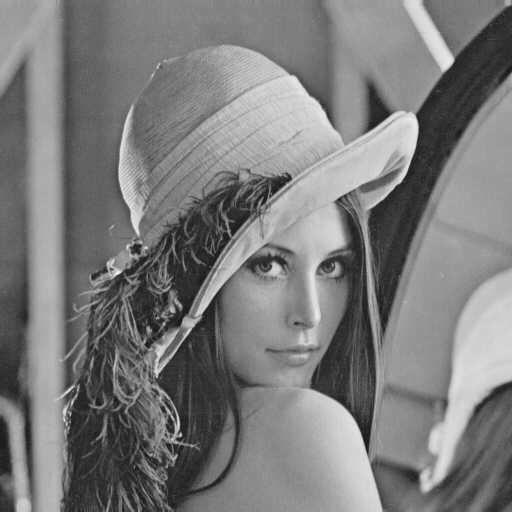
\includegraphics[width=0.45\linewidth]{question4/jpeg_Z1}
	}
	\subfigure[JPEG Z3; PSNR +8.22dB]{
	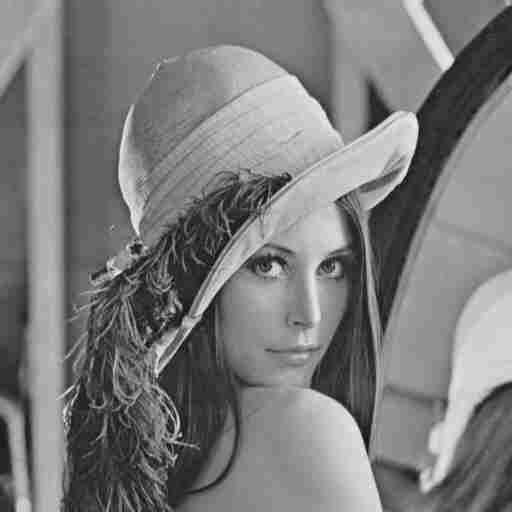
\includegraphics[width=0.45\linewidth]{question4/jpeg_Z3}
	}
	\subfigure[JPEG Z5; PSNR +6.31dB]{
	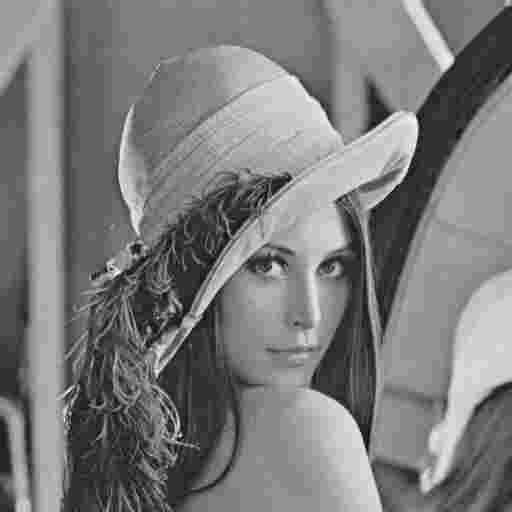
\includegraphics[width=0.45\linewidth]{question4/jpeg_Z5}
	}
	\subfigure[JPEG Z1; PSNR +3.25dB]{
	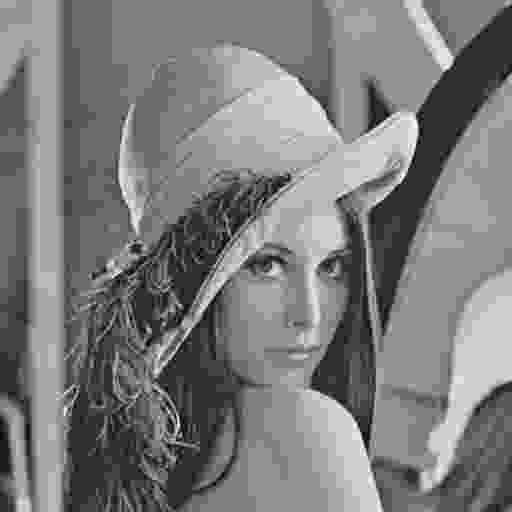
\includegraphics[width=0.45\linewidth]{question4/jpeg_Z10}
	}

\end{figure}

